%%%%%%%%%%%%%%%%%%%%%%%%%%%%%%%%%%%%%
%Presentazione esame di Dottorato Davide Spataro
%opencal.tex
%Purpose: This file describes Opencal: its scope, API showing an example (fractal or game of life or sciddica)
%@author Davide Spataro
%@version 1.0 14/01/2018 Eindhoven
%%%%%%%%%%%%%%%%%%%%%%%%%%%%%%%%%%%%

\section{OpenCAL - The Open Computing Abstraction Layer for Extended Cellular Automata and The Finite Difference Method}
\subsection[OpenCAL]{Features} 
\frame{\frametitle{OpenCAL} 
	\begin{block}{OpenCAL - Features}
		\begin{itemize}
			\item Seamless parallel programming of CA and FDM solvers
			\item API + libraries + Domain Specific Language
			\item Transparent Built-in Optimizations
			\item Open-source\footnote{https://github.com/OpenCALTeam/opencal}
		\end{itemize}
	\end{block}
	\begin{block}{Write once $\Longrightarrow$ executes everywhere}			
		\begin{itemize}
			\item Serial
			\item Multi-threaded
			\item \textbf{single}-GPU/FPGA/MIC
			\item \textbf{multi}-GPU/FPGA/MIC
			\item Distributed-memory + \textbf{multi}-GPU/FPGA/MIC
		\end{itemize}
	\end{block}
}
%%%%%%%%%%%%%%%%%%%%%%%%%%%%%%%%%%%%
\frame{\frametitle{OpenCAL - Architecture}
	\begin{figure}
		\centering
		\includegraphics[width=1.1\textwidth]{images/Figure05}
	\end{figure}
}
%%%%%%%%%%%%%%%%%%%%%%%%%%%%%%%%%%%%
\frame{\frametitle{OpenCAL - API} 
	\begin{block}{High Level API is simple}
		\begin{itemize}
			\item Model Definition (size, neighborhood, optimizations)
			\item Run parameters (iterations, implicit or explicit $t+1$ update)
			\item Data Definition and initialization
			\item Definition of per grid point function (e.g. forward Explicit or custom)
			\item Steering functions (per grid e.g. average, or custom) 
			\item API + libraries + Domain Specific Language
		\end{itemize}
	\end{block}
	
}

%------------------------------------------------------------------------------

\begin{frame}{OpenCAL developing process}

In order to define the CCA, the user needs to

\begin{itemize}
	\item Define a CA object and initialize its parameters
	\begin{itemize}
		\item Domain dimensiona/size
		\item Type of neighborhood
		\item Boundary conditions
		\item Type of optimization (if any)
	\end{itemize}
	\item Define a simulation object and initialize its parameters
	\begin{itemize}
		\item The model to use
		\item Number of iterations
	\end{itemize}
	\item Define substates
	\item Define transition function\textit{s}
	\item Optionally, the user can define the following global functions
	\begin{itemize}
		\item initialization function
		\item steering function (per grid e.g. average or custom)
	\end{itemize}
\end{itemize}

\end{frame}

%%%%%%%%%%%%%%%%%%%%%%%%%%%%%%%%%%%%
\begin{frame}[fragile]
\frametitle{OpenCAL - Heat Equation example - 1} 
\centering\textbf{Minimal Example: Driver Code}
  \begin{lstlisting}[numbers=none]
//Grid of 256^3 points
model = calCADef3D(256, 256, 256, CAL_MOORE_NEIGHBORHOOD_3D,...)
simulation = calRunDef3D(model, 1, STEPS,...)
//add substates
Q_T = calAddSubstate3Dr(heatModel)
//add transition function
calAddElementaryProcess3D(model,EulerForward)
//run the simulation
calRun3D(simulation)
// Save the substate to file
calSaveSubstate3Dr(model, Q_T, "./output.txt")
calRunFinalize3D(simulation)
calFinalize3D(model);
\end{lstlisting}
\end{frame}
%%%%%%%%%%%%%%%%%%%%%%%%%%%%%%%%%%%%
\begin{frame}[fragile]
\frametitle{OpenCAL - Heat Equation example - 2} 
\centering\textbf{Minimal Example: Per Cell Code}
\begin{lstlisting}[numbers=none]

void EulerForward(CALModel3D* model,int i,int j,int k){
//current cell temperature value
CALreal cv =calGet3Dr(model, Q_T ,i,j,k )
CALreal dx2 = (calGet3Dr(model, Q_T ,i+1,j,k) +calGet3Dr(model,Q_T,i-1,j,k) - (2*cv))/(DELTA_X*DELTA_X)

CALreal dy2 = (calGet3Dr(model,Q_T ,i,j+1,k) + calGet3Dr(heatModel,Q_T ,i,j-1,k) - (2*cv))/(DELTA_Y*DELTA_Y);

CALreal dz2 = (calGet3Dr(model,Q_T ,i,j,k+1) + calGet3Dr(heatModel,Q_T ,i,j,k-1) - (2*cv))/(DELTA_Z*DELTA_Z);

CALreal newValue = currValue + DELTA_T*THERMAL_DIFFUSIVITY_WATER * (dx2 + dy2 +dz2);
//set new temperature
calSet3Dr(heatModel, Q_T, i, j, k, newValue);

\end{lstlisting}
\end{frame}


%%%%%%%%%%%%%%%%%%%%%%%%%%%%%%%%%%%%
\begin{frame}[fragile]
\frametitle{OpenCAL - Domain Decomposition} 
	\begin{block}{Cluster File}
		The user can specify which portion of the domain goes executed where.
		OpenCAL uses a configuration file that specifies
		\begin{itemize}
			\item list of nodes and for each of them its workload
			\item a list of accelerators to be used on that node
			\item each GPU gets assigned its workload
		\end{itemize}
	\end{block}
\begin{lstlisting}[numbers=none, basicstyle=\small]
16384 16384
2
10.0.0.111 2
0 0 4096
0 1 4099
10.0.0.222 3
0 0 1200
1 0 3200
1 1 3792
\end{lstlisting}
\end{frame}


\frame{\frametitle{Domain Decomposition/Boundaries Exchange}
	\centering
	The domain is partitioned among devices along the first dimension listed in the configuration file
	\begin{figure}
		\centering
		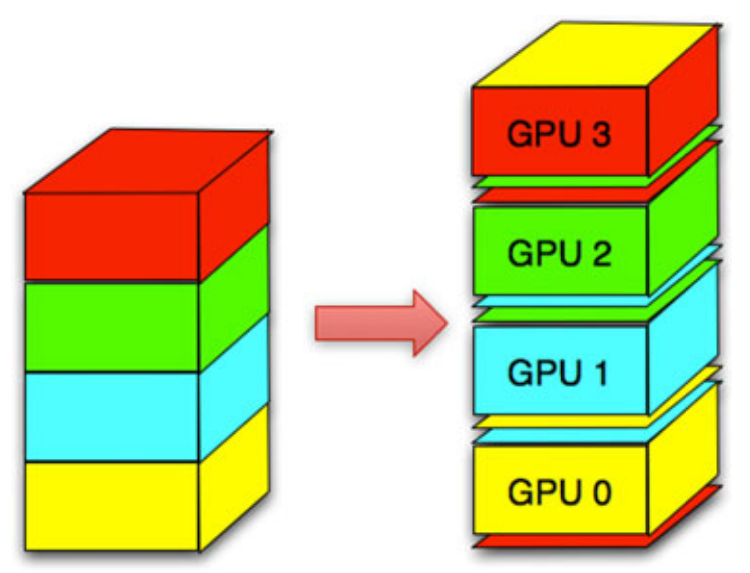
\includegraphics[width=1\textwidth]{images/multigpu_domain_decomposition}
	\end{figure}
	
}

\frame{\frametitle{Domain Decomposition/Boundaries Exchange}
	\begin{figure}
		\centering
		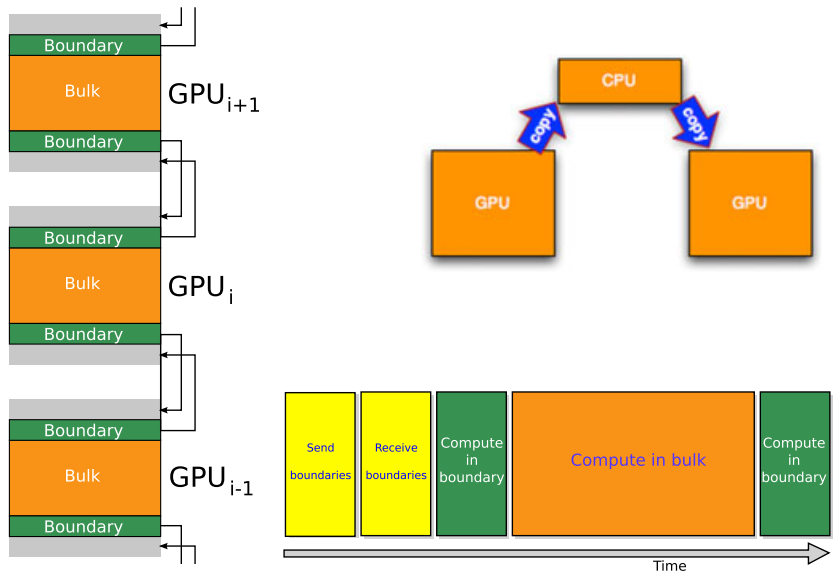
\includegraphics[width=1\textwidth]{images/multigpu_naive_exchange}
	\end{figure}
	
}


